\documentclass[a4paper,12pt]{article}
\usepackage{graphicx}
\usepackage{amsmath}
\usepackage{float}
\usepackage{hyperref}
\usepackage{geometry}
\usepackage{listings}
\usepackage{xcolor}
\geometry{top=1in, bottom=1in, left=1in, right=1in}

% Define colors for a fresh, readable style
\definecolor{keywordcolor}{RGB}{0, 102, 204}   % Keywords (blue)
\definecolor{stringcolor}{RGB}{183, 28, 28}    % Strings (red)
\definecolor{commentcolor}{RGB}{85, 107, 47}  % Comments (green)
\definecolor{bgcolor}{RGB}{245, 245, 245}      % Light gray background
\definecolor{numbercolor}{RGB}{150, 150, 150}  % Line numbers

% Configuration for code listings
\lstset{
    backgroundcolor=\color{bgcolor},     % Background color
    basicstyle=\ttfamily\footnotesize,   % Code font and size
    keywordstyle=\color{keywordcolor}\bfseries, % Bold keywords
    stringstyle=\color{stringcolor},     % String color
    commentstyle=\color{commentcolor}\itshape, % Italic comments
    numberstyle=\color{numbercolor}\tiny, % Line numbers
    numbers=left,                        
    stepnumber=1,                        
    breaklines=true,                     
    showstringspaces=false,              
    frame=single,                        
    rulecolor=\color{gray},              % Frame color
    tabsize=4,
    captionpos=b,                        
    xleftmargin=1em,
    framexleftmargin=0em,
}

\title{Implementation and Performance Analysis of Bitonic Sort using CUDA}

\author{
    \small Aristotle University of Thessaloniki - Department of Electrical and Computer Engineering \\[0.5em]
    \small Parallel and Distributed Systems\\[1.5em]
    Koumparidou Eleni and Maria Sotiria Kostomanolaki \\[1em]
}
\date{January 2025}

\begin{document}

\maketitle

\begin{abstract}
This project implements a parallel sorting algorithm using \textbf{CUDA}, based on the Bitonic Sort algorithm. The goal is to explore different strategies for parallelizing the Bitonic Sort algorithm using CUDA. The program sorts $N = 2^q$ integers in ascending order, leveraging GPU parallelism to accelerate the sorting process. Three versions of the algorithm have been developed (V0, V1, V2), each one using a different aspect of parallelism (thread-level parallelism, kernel synchronization, shared memory usage).. Each implementation aims to improve the usage of CUDA's resources using different CUDA features to achieve high-performance and higher speed sorting. The correctness and the execution time of this algorithm for different input sizes ($q \in [20, 27]$) are compared to the quickSort (\texttt{qSort}) algorithm, implemented in C. Performance tests on the Aristotelis cluster highlight the speedup achieved by GPU parallellism and demonstrate the impact of CUDA on sorting efficiency.
\end{abstract}

\tableofcontents

\section{Introduction}
Before presenting the implementation, we provide an overview of the Bitonic Sort algorithm and the optimization approaches explored in this assignment. Three progressively improved versions of the algorithm are introduced, each leveraging CUDA's capabilities to enhance sorting performance.


\subsection{Background: Bitonic Sort Algorithm}  
\textbf{Bitonic Sort} is a sorting algorithm that recursively transforms an unsorted sequence into a bitonic sequence. A \textbf{bitonic sequence} is a sequence of numbers that first monotonically increases and then monotonically decreases (or vice versa). It consists of two main steps: 
\begin{enumerate}
 \item \textbf{Bitonic Merge:} This step takes a bitonic sequence and produces a fully sorted sequence by separating the elements into two subsequences containing minima and maxima, based on elementwise comparisons. The process is recursively repeated for each half. The time complexity of Bitonic Merge is \(O(n \log n)\).  

\item \textbf{Bitonic Sort:} This recursively divides the input sequence, sorting one half in ascending order and the other in descending order to form a bitonic sequence. Bitonic Merge is then applied to produce the final sorted result. The overall time complexity of Bitonic Sort is \(O(n (\log n)^2)\).  
\end{enumerate}
For the C implementation of the serial algorithm and a visualization, you can refer to the following excellent resource \cite{sortvisualizer}.

\subsubsection*{Key Terms}
The following key terms will be used throughout the report:
\begin{itemize}
    \item \textbf{\texttt{group\_size}}: It represents the amount of elements from the array that will follow the same sorting pattern for each pass of the Bitonic Sort algorithm. Initially set to 2, the \texttt{group\_size} doubles with each iteration until the whole array is sorted.
    \item \textbf{\texttt{distance}}: The gap between elements that need to be compared during each sorting step. In every sorting phase of the algorithm distance is taking the following values:
    \[
    \left[ \frac{\text{group\_size}}{2}, \dots, 2, 1 \right]
    \]
    \item \textbf{partner}: The element that needs to be compared with the chosen element. 
    \item \textbf{threads}: Individual units within a CUDA block. Threads work in parallel to process elements in the array.
    \item \textbf{blocks}: Groups of threads in CUDA. A block can hold up to 1024 threads, and the threads within a block cooperate to perform part of the sorting task.
\end{itemize}

\subsection{CUDA Memory Model Overview}
In this implementation, different versions of the algorithm utilize different types of CUDA memory (see Figure \ref{fig:CUDA}) to optimize performance:  

\begin{itemize}  
    \item \textbf{Global Memory}: Used in Versions 0 and 1. It is accessible by all threads across all blocks but has high latency.
    \item \textbf{Shared Memory}: Introduced in Version 2. Shared memory is only accessible within a block, requiring careful data management.  
\end{itemize}  

\begin{figure}[H]
    \centering
    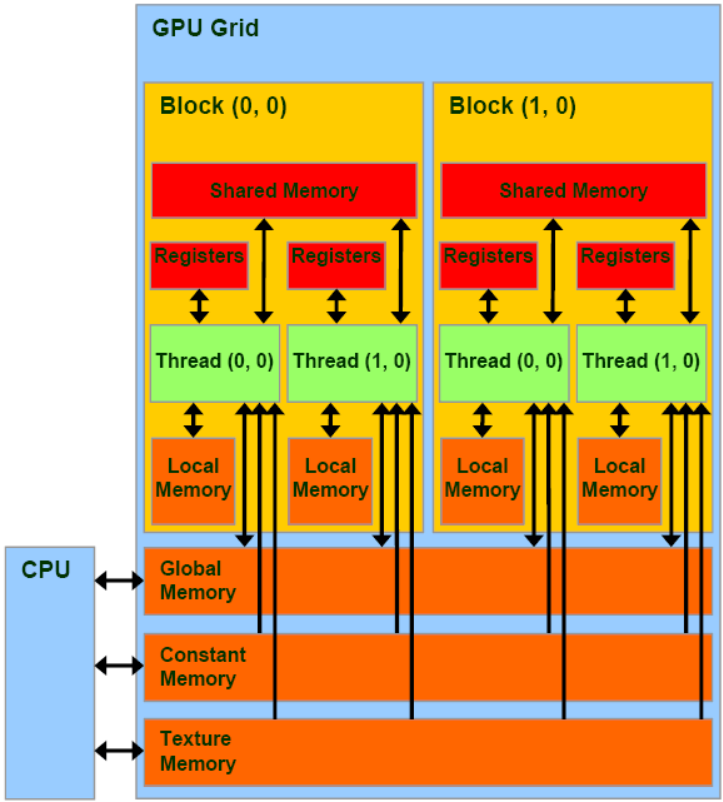
\includegraphics[width=0.5\linewidth]{assets/CUDA Memory Model.png}
    \caption{CUDA Memory Model}
    \label{fig:CUDA}
\end{figure}

\section{Algorithm Description}

The main function of the implementation starts by allocating memory on both the CPU and GPU for an array of size \(2^q\), where \(q\) is specified by the user at the \texttt{make run} command and ranges from 20 to 27. This dual memory allocation is essential because the CPU and GPU have separate memory spaces. A CPU (host) function can only access CPU memory, while GPU functions (kernels) can only access GPU memory. Therefore, two separate arrays are required: one on the CPU and one on the GPU. 

After memory allocation, the CPU array is initialized with random integers, and the data is copied to the GPU. The function \texttt{bitonicSort()} is then called to sort the elements. The implementation of this function varies depending on the selected version (V0, V1, or V2). 

Once the sorting operation is completed, the results are copied back to the CPU. Finally, the program evaluates the correctness of the sorting operation and calculates the execution time.

The following subsections describe the differences between each version of the algorithm and the CUDA features utilized.

\subsection{V0: Basic Parallel Implementation}

Version 0 implements the Bitonic Sort algorithm using the fundamentals of parallel programming in CUDA. This version introduces a straightforward approach to parallel sorting using GPU threads.
The main idea is to assign in each thread the task of \textbf{comparing} and potentially swapping two elements in the array. This is done using the \texttt{exchange\_V0} kernel function in Listing \ref{lst:exchangeV0}.
\\
\begin{lstlisting}[language=C, caption={Exchange process using GPU's threads}, label={lst:exchangeV0}]
    __global__ void exchange_V0(int *array, int size, int group_size, int distance) {
    int tid = threadIdx.x + blockIdx.x * blockDim.x;
    int idx = (tid / distance) * distance * 2 + (tid % distance);
    int partner = idx ^ distance;
    bool sort_descending = idx & group_size;

    if (idx < size && partner < size && idx < partner){ 
        if (!sort_descending && array[idx] > array[partner]){
            swap(array, idx, partner);  // keep min elements   }
        if (sort_descending && array[idx] < array[partner]) {
            swap(array, idx, partner);   // keep max elements  }
    }
}
\end{lstlisting}
To call the previous kernel we use the maximum number of threads, 1024, and the blocks that are needed to manage all the elements of the array. These parameters are definied in \texttt{bitonicSort} function in Listing \ref{lst:bitonicV0}.
\\
\begin{lstlisting}[language=C, caption={Kernel call for elementwise comparison using threads}, label={lst:bitonicV0}]
void bitonicSort(int *array, int size)
{
    // GPU PARAMETERS
    int threads_per_block = 1024;  
    int blocks_per_grid = size / threads_per_block; 

    for (int group_size = 2; group_size <= size; group_size <<= 1){ 
        for (int distance = group_size >> 1; distance > 0; distance >>= 1)
            exchange_V0<<<blocks_per_grid, threads_per_block>>>(array, size, group_size, distance);}
    }
\end{lstlisting}

\subsubsection*{Index Calculation}

A critical aspect of this approach is to assign elements to threads by calculating the array index (\texttt{idx}) as a function of the current thread ID (\texttt{tid}). This management is not handled by CUDA, so it is calculated by the following expression:
\\
\begin{lstlisting}[language=C]
int idx = (tid / distance) * distance * 2 + (tid % distance);
\end{lstlisting}
\newpage
Here is a breakdown of the formula:
\begin{itemize}
    \item \texttt{(tid / distance)}: Computes which block the thread belongs to for this particular step of the sorting process.
    \item \texttt{* distance * 2}: Takes into consideration the fact that comparisons are made between pairs separated by twice the \texttt{distance}.
    \item \texttt{(tid \% distance)}: Identifies the thread’s relative position within its block.
\end{itemize}

This formula guarantees a unique index for each thread, ensuring that every element in the array is correctly mapped for comparison during each stage of the Bitonic Merge process.

\subsubsection*{Swapping Elements on the GPU}

The swap of two elements is an important and often part of sorting. On the GPU, swaps are performed using the following device function:
\\
\begin{lstlisting}[language=C]
__device__ void swap(int *array, int idx, int partner) {
    int temp;
    temp = array[idx];
    array[idx] = array[partner];
    array[partner] = temp;
}
\end{lstlisting}


\subsubsection*{Synchronization Overhead}

In this version, every kernel call requires global synchronization across the GPU, which can be really "expensive" in terms of time. The processing must wait for all threads to finish their comparisons and swaps before proceeding to the next distance in the sorting step. The improvement of this delay is the goal for the next version (V1), which addresses this with the use of local block synchronization.

\subsection{V1: Local Block Synchronization}

Version 1 aims to improve the execution time of the algorithm developed in Version 0 by reducing the global synchronization overhead. To achieve this, we take advantage of the local block synchronization, in which the threads inside the same block can be synchronized at a lower cost. 

The main idea is that, when the array fits within a single block, we can process all the required exchanges for a given group\_size with \textbf{a single kernel call}. For example, if the array contains 2048 elements, we need to perform 1024 comparisons. In Version 0, this would involve multiple kernel launches, each handling a specific \texttt{distance}. In Version 1, the entire sorting operation for that \texttt{group\_size} can be completed in a single kernel call, significantly reducing synchronization overhead. To achieve this we introduce the \texttt{exchange\_V1} kernel. 

\subsubsection*{Sorting Overview}
In order to use the property mentioned before, \texttt{bitonicSort} is modified to use the following three kernels, also shown in Listing \ref{lst:bitSort1}:

\begin{itemize}
    \item \textbf{Initial sorting}: We make the exchanges for all groups of size less than 2048 using \texttt{initialExchange}. 
    \item \textbf{Exchanges for distances greater than 1024}: After the initial sorting, when the groups become larger than 2048 and the distances become greater than 1024 we use \texttt{exchange\_V0} kernel (implemented in Version 0) to handle large distances ($>$1024).
    \item \textbf{Exchanges for distances smaller than 1024}: Following the case explained above, we use the \texttt{exchange\_V1} kernel to handle small distances ($<$=1024).
    
\end{itemize}

\begin{lstlisting}[caption={Bitonic Sort algorithm of V1}, label={lst:bitSort1}]
    __host__ void bitonicSort(int *array, int size)
{
    // GPU PARAMETERS
    int threads_per_block = 1024;
    int blocks_per_grid = size / threads_per_block;

    initialExchange<<<blocks_per_grid, threads_per_block>>>(array, size);

    for (int group_size = 4096; group_size <= size; group_size <<= 1)
    { // group_size doubles in each reccursion

        for( int distance = group_size >> 1; distance > 1024; distance >>=1)
        {
            // Handle large distances (>1024)
            exchange_V0<<<blocks_per_grid, threads_per_block>>>(array, size, group_size, distance);
        }

        // Handle small distances (<=1024)
        exchange_V1<<<blocks_per_grid, threads_per_block>>>(array, size, group_size);
    }
}
\end{lstlisting}

\subsubsection*{Initial Exchange}
As mentioned before, the algorithm starts by sorting small group sizes and doubles the \texttt{group\_size} until it reaches the full size of the array.This means that we can sort all groups until the group consists of 2048 elements optimally, because the distance will never exceed 1024, thus fulfilling the local block synchronization requirement. This is done using a single call of the \texttt{initialExchange} kernel function presented in Listing \ref{lst:initExchange}. 

In this implementation, we call the \texttt{\_\_syncthreads()} function after each exchange to ensure that all threads within a block have completed their operations and are working with the latest data.
\\
\begin{lstlisting}[ caption={Initial Exchange}, label={lst:initExchange}]
__global__ void initialExchange(int *array, int size)
{
    int tid = threadIdx.x + blockIdx.x * blockDim.x;

    for (int group_size = 2; group_size <= 2048; group_size <<= 1)
    {
        for (int distance = group_size >> 1; distance > 0; distance >>= 1)
        {
            int idx = (tid / distance) * distance * 2 + (tid % distance);
            int partner = idx ^ distance;
            bool sort_descending = idx & group_size;

            if (idx < size && partner < size && idx < partner)
            { // ensure bounds are checked before accessing array

                if (!sort_descending && array[idx] > array[partner])
                {
                    // keep min elements
                    swap(array, idx, partner);
                }
                if (sort_descending && array[idx] < array[partner])
                {
                    // keep max elements
                    swap(array, idx, partner);
                }

                __syncthreads();
            }
        }
    }
}
\end{lstlisting}

Once this kernel completes its execution, the next step of the Bitonic Sort doubles the group size, exceeding 2048 elements. At this stage (4096), the distance starts at 2048, requiring 2048 threads for the exchange process, which are now divided into two blocks, making us rely on global memory for coordination. From this point forward, and until the array is fully sorted, large distances (>1024) will be handled by \texttt{exchange\_V0} and smaller distances (<=1024) by \texttt{exchange\_V1}.

\subsubsection*{V1 Exchange}

Version 1 operates similarly to the initial exchange phase of the algorithm, with one key difference: it takes \texttt{group\_size} as an input to determine whether elements should be sorted in ascending or descending order, therefore eliminating the outer \texttt{for} loop.  

The remaining \texttt{for} loop is the main improvement over Version 0, as Version 1 performs all exchanges for distances up to 1024 within a single kernel call, as shown in Listing \ref{lst:V1_ex}. A \texttt{\_\_syncthreads()} call is placed after every exchange to ensure that all threads within a block have completed their exchanges before proceeding to the next.
\newpage
\begin{lstlisting}[caption={V1 Exchange algorithm}, label={lst:V1_ex}]  
__global__ void exchange_V1(int *array, int size, int group_size)
{
    int tid = threadIdx.x + blockIdx.x * blockDim.x;

    for (int distance = 1024; distance > 0; distance >>= 1)
    {
        int idx = (tid / distance) * distance * 2 + (tid % distance);
        int partner = idx ^ distance;
        bool sort_descending = idx & group_size;

        if (idx < size && partner < size && idx < partner)
        { // ensure bounds are checked before accessing array

            if (!sort_descending && array[idx] > array[partner])
            {
                // keep min elements
                swap(array, idx, partner);
            }
            if (sort_descending && array[idx] < array[partner])
            {
                // keep max elements
                swap(array, idx, partner);
            }

            __syncthreads();
        }
    }
}
\end{lstlisting}

\subsubsection*{Global Memory Latency}

Although Version 1 reduces synchronization overhead by utilizing local block synchronization, it still relies entirely on global memory for data access. Since global memory has high latency, frequent memory accesses can slow down performance. The goal of the next version (V2) is to address this issue by utilizing shared memory, which allows faster data exchange within thread blocks and reduces the need for costly global memory accesses.

\subsection{V2: Shared Memory Optimization}
Version 2 builds upon the optimizations introduced in V1 by utilizing \textbf{CUDA’s shared memory}.

\subsubsection*{Shared Memory}
Shared memory in CUDA is accessible by all threads within a block. Compared to global memory, shared memory provides faster access. In fact, shared memory latency is roughly 100x lower than uncached global memory latency when no bank conflicts occur. 

To access an array through shared memory, we have to make a copy of the array from global memory to shared memory. We use three key variables:
\begin{itemize}
    \item \textbf{Local Thread Id}: The Id of a thread in shared memory.
    \item \textbf{Global Thread Id}: The position of an element in the global array.
    \item \textbf{Offset}: The number of elements to skip in the global array because they belong to a different block, as each block loads 2048 consecutive elements into shared memory.
\end{itemize}

\begin{lstlisting}
    int local_tid = threadIdx.x;
    int global_tid = local_tid + blockIdx.x * blockDim.x;
    int offset = blockIdx.x * blockDim.x * 2;
\end{lstlisting}
To copy the data to and from shared memory, we use the two helper functions as shown in Listing \ref{lst:transfer}. The functions \texttt{load\_global\_to\_local} and \texttt{load\_local\_to\_global} handle the transfer of data between global and shared memory. By utilizing the variables explained above, we ensure that each block loads its specific 2048 elements from the global memory into shared memory correctly without overlap and vice versa.
\\
\begin{lstlisting} [caption={Algorithm to handle transfer of data}, label={lst:transfer}]
__device__ void load_global_to_local(int *array, int *local_array, int size, int local_tid, int offset)
{
    if (local_tid + offset < size && local_tid + offset + blockDim.x < size)
    {
        local_array[local_tid] = array[local_tid + offset];
        local_array[local_tid + blockDim.x] = array[local_tid + offset + blockDim.x];

        __syncthreads();
    }
}

__device__ void load_local_to_global(int *array, int *local_array, int size, int local_tid, int offset)
{
    if (local_tid + offset < size && local_tid + offset + blockDim.x < size)
    {
        array[local_tid + offset] = local_array[local_tid];
        array[local_tid + offset + blockDim.x] = local_array[local_tid + blockDim.x];

        __syncthreads();
    }
}
\end{lstlisting}

\subsubsection*{Initial and V2 Exchange}
To take advantage of shared memory, we modify both the \texttt{initialExchange} and \texttt{exchange\_V1} kernels. Specifically, we adjust the \texttt{initialExchange} from Version 1 to compute the index of the local array in shared memory using the previously explained parameters and formulas. It is important to calculate both the \texttt{global\_idx} and \texttt{idx} (local) values: \texttt{global\_idx} uses the \texttt{global\_tid}, while \texttt{idx} uses the \texttt{local\_tid}. The \texttt{idx} is used to determine the partner element within the same block, whereas the sorting order is still determined by the position in the global array (using \texttt{global\_idx}).
\\
\begin{lstlisting}
    int global_idx = (global_tid / distance) * distance * 2 + (global_tid % distance);
    int idx = (local_tid / distance) * distance * 2 + (local_tid % distance);
    int partner = idx ^ distance;
    bool sort_descending = global_idx & group_size;
\end{lstlisting}
The same strategy is followed in \texttt{exchange\_V2} to load the array in shared memory and to access the right elements determined by the Bitonic Sort algorithm.

\section{Performance Analysis}
To evaluate the efficiency of the implemented versions (V0,V1,V2) at a large scale, we performed testing on the GPU partition of the \textbf{Aristotelis Cluster}, using a \textbf{NVIDIA Tesla P100} GPU.

\subsection{Execution Time}
All versions (V0, V1, V2) were tested on varying input sizes, specifically for \( q = [20:27] \) elements, to assess scalability and performance against the qSort algorithm. As shown in Figure \ref{fig:qSort}, leveraging CUDA provides a significant speedup across all versions when compared to qSort, particularly as the number of elements increases. This highlights the substantial efficiency gains achieved through parallelization on the GPU.

\begin{figure}[H]
    \centering
    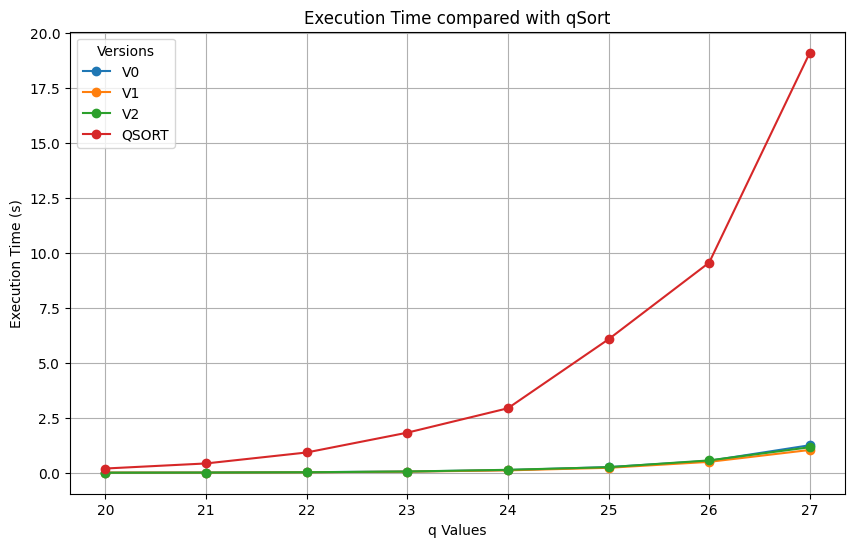
\includegraphics[width=0.8\linewidth]{assets/execution_time_qsort.png}
    \caption{Execution time compared with qSort}
    \label{fig:qSort}
\end{figure}

Additionally, in Figure \ref{fig:versions}, we observe the impact of the different optimization techniques implemented across the versions. While Version 2 introduces shared memory optimization and delivers better performance than V0, it is slower than V1. This slowdown in Version 2 can likely be attributed to the overhead of memory copying and synchronization between global and shared memory, which, while reducing latency in many cases, also introduces additional complexity in certain configurations. Despite our efforts to further optimize, this trade-off in execution time persists, and unfortunately, we were unable to fully overcome this challenge to achieve faster execution than V1.

\begin{figure}[H]
    \centering
    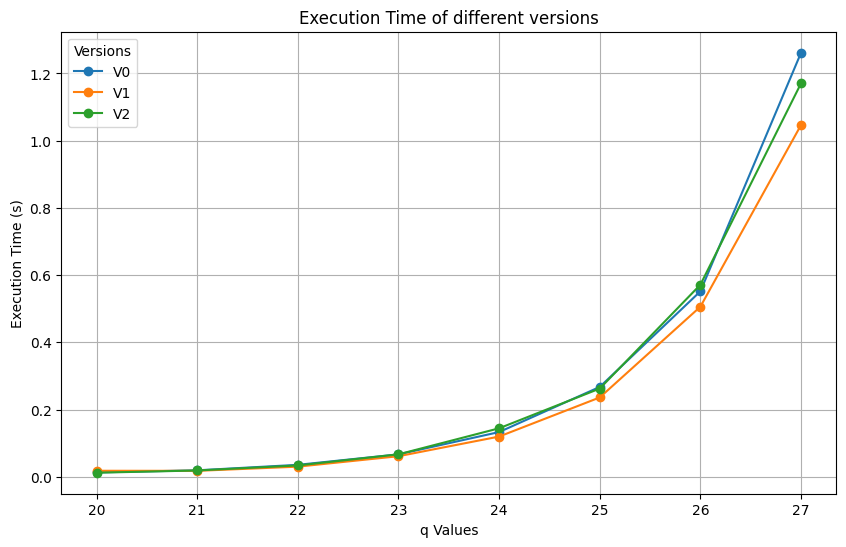
\includegraphics[width=0.8\linewidth]{assets/execution_time_versions.png}
    \caption{Execution times of different versions}
    \label{fig:versions}
\end{figure}

In summary, the specific optimizations introduced by the different versions that result in the above execution time acceleration are:

\begin{itemize}
    \item \textbf{V0}: The baseline version that uses basic parallelization with CUDA, offering a significant speedup over the qSort implementation due to the parallel nature of the algorithm. Despite lacking advanced optimizations, V0 outperforms qSort by a large margin.
    \item \textbf{V1}: Implements global synchronization optimizations, further reducing execution time compared to V0 by minimizing unnecessary waiting between threads.
    \item \textbf{V2}: Utilizes shared memory to improve data access, but its performance is slightly hindered by synchronization overhead, making it slower than V1 in certain cases.
\end{itemize}

\subsection{Speedup}
Figure \ref{fig:speedup} shows the acceleration of each version in comparison to qSort. Version V1 demonstrates the most significant acceleration, benefiting from the optimizations introduced, while Version V2, despite using shared memory, shows a slight performance drop compared to V1. This suggests that while shared memory can improve efficiency in some contexts, other factors like synchronization overhead or thread management may limit its overall performance in this case.

\begin{figure}[H]
    \centering
    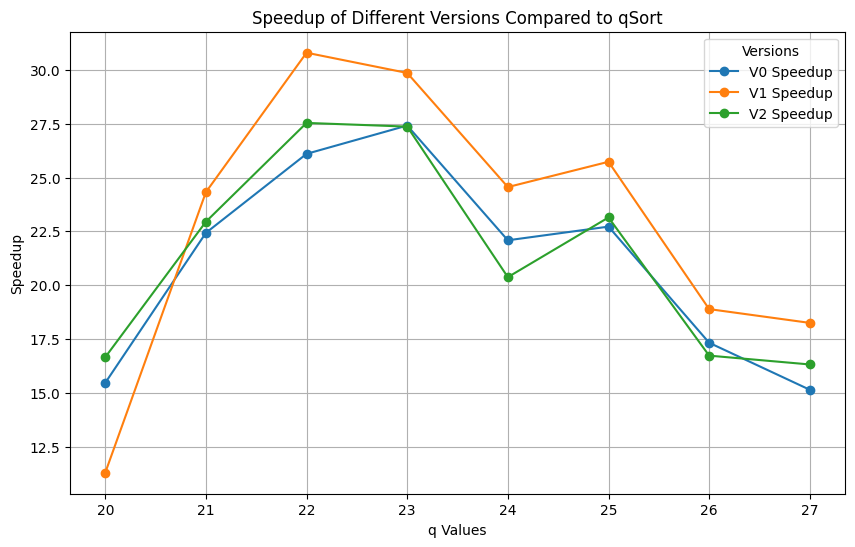
\includegraphics[width=0.8\linewidth]{assets/speedup.png}
    \caption{Speedup from qSort}
    \label{fig:speedup}
\end{figure}

\section{Conclusion}
In conclusion the implementation of Bitonic Sort with CUDA has a significant improvement in execution time and can be extremely effective when handling large datasets. By leveraging parallel processing capabilities of the GPU, the CUDA implementation vastly outperforms the sequential qSort, with further improvements observed in the optimized versions. The results underscore the effectiveness of utilizing GPU to enhance the scalability and performance of sorting algorithms.

\section*{GitHub repository}
You can find the full source code of our implementation in this \href {https://github.com/ekoumpar/bitonicSort_CUDA/tree/main}{Github repository}.

\begin{thebibliography}{9}

\bibitem{sortvisualizer} \textit{Bitonic Sort Visualization}. Available \href{https://www.sortvisualizer.com/bitonicsort/}{here}.
\bibitem{shared memory} \textit{Shared Memory in CUDA}. Available 
\href{https://developer.nvidia.com/blog/using-shared-memory-cuda-cc/}{here}
\bibitem{CUDA picture} \textit{CUDA Memory Model}. Available \href{https://www.3dgep.com/cuda-memory-model/}{here}.
\end{thebibliography}

\section*{Acknowledgments}
We would like to acknowledge the use of ChatGPT for assisting in editing parts of this report for clarity, as well as GitHub Copilot for its support in generating Python plotting scripts that contributed to the creation of the result figures.

\end{document}